\documentclass[12pt]{article}

% a template that a friend gave, it's worked well enough for me
% i have added some packages and stuff that have proved useful

\usepackage{fancyhdr}
\usepackage{tipa}
\usepackage{fontspec}
\usepackage{amsfonts}
\usepackage{enumitem}
\usepackage[margin=1in]{geometry}
\usepackage{graphicx}
\usepackage{float}
\usepackage{amsmath}
\usepackage{braket}
\usepackage{amssymb}
\usepackage{booktabs}
\usepackage{hyperref}
\usepackage{mathtools}
\usepackage{xcolor}
\usepackage{float}
\usepackage{algpseudocodex}
\usepackage{titlesec}
\usepackage{bbm}

\pagestyle{fancy}
\fancyhf{} % sets both header and footer to nothing
\lhead{Kevin Sheng}
\setmainfont{Comic Neue}
\renewcommand{\headrulewidth}{1pt}
\setlength{\headheight}{0.75in}
\setlength{\oddsidemargin}{0in}
\setlength{\evensidemargin}{0in}
\setlength{\voffset}{-.5in}
\setlength{\headsep}{10pt}
\setlength{\textwidth}{6.5in}
\setlength{\headwidth}{6.5in}
\setlength{\textheight}{8in}
\renewcommand{\headrulewidth}{0.5pt}
\renewcommand{\footrulewidth}{0.3pt}
\setlength{\textwidth}{6.5in}
\usepackage{setspace}
\usepackage{multicol}
\usepackage{float}
\setlength{\columnsep}{1cm}
\setlength\parindent{24pt}
\usepackage [english]{babel}
\usepackage [autostyle, english = american]{csquotes}
\MakeOuterQuote{"}

\setlength{\parskip}{6pt}
\setlength{\parindent}{0pt}

\titlespacing\section{0pt}{12pt plus 4pt minus 2pt}{0pt plus 2pt minus 2pt}
\titlespacing\subsection{0pt}{12pt plus 4pt minus 2pt}{0pt plus 2pt minus 2pt}
\titlespacing\subsubsection{0pt}{12pt plus 4pt minus 2pt}{0pt plus 2pt minus 2pt}

\hypersetup{colorlinks=true, urlcolor=blue}

\newcommand{\correction}[1]{\textcolor{red}{#1}}


\rhead{Math 180}

\makeatletter
\def\@seccntformat#1{%
  \expandafter\ifx\csname c@#1\endcsname\c@section\else
  \csname the#1\endcsname\quad
  \fi}
\makeatother

\begin{document}

\section{Chapter 4.1}

\begin{enumerate}
      \item[1] \begin{enumerate}
                  \item I've provided a valid node relabelling below:
                        \begin{center}
                              \hfill
                              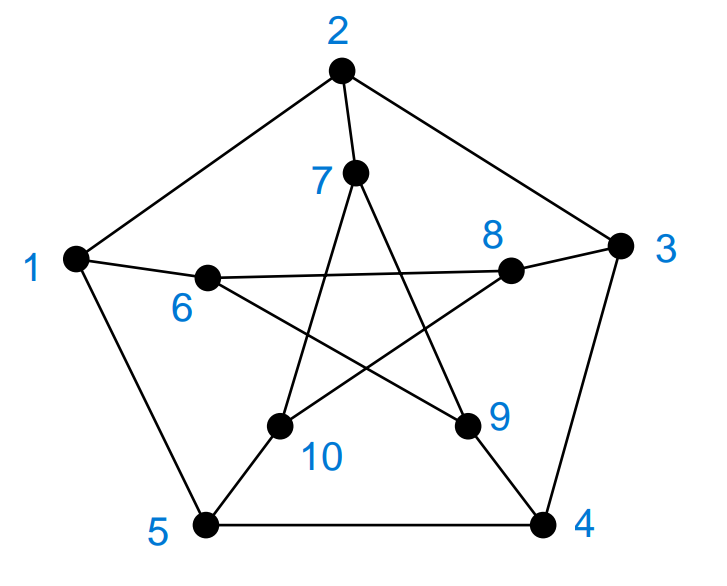
\includegraphics[width=5cm]{img/hw1/iso1}
                              \hfill
                              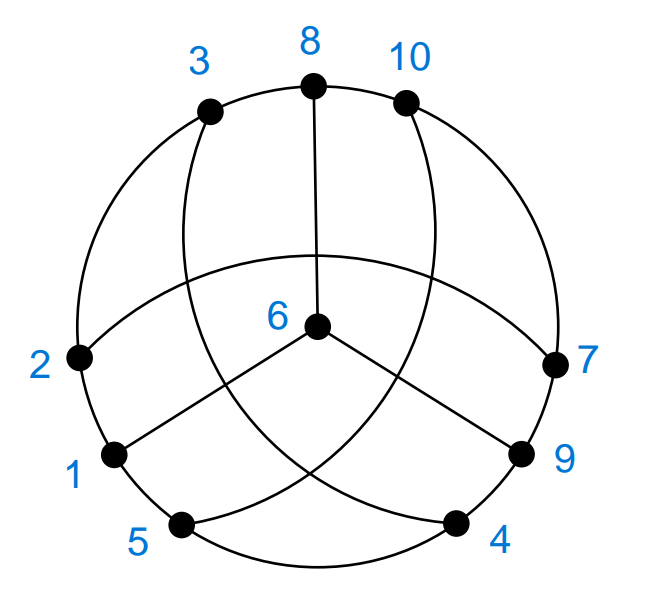
\includegraphics[width=5cm]{img/hw1/iso2}
                              \hfill \mbox{}
                        \end{center}
                  \item Here's another node relabelling, this time with sets.
                        For consistency, I've written each set as a sorted ordered pair.
                        \begin{center}
                              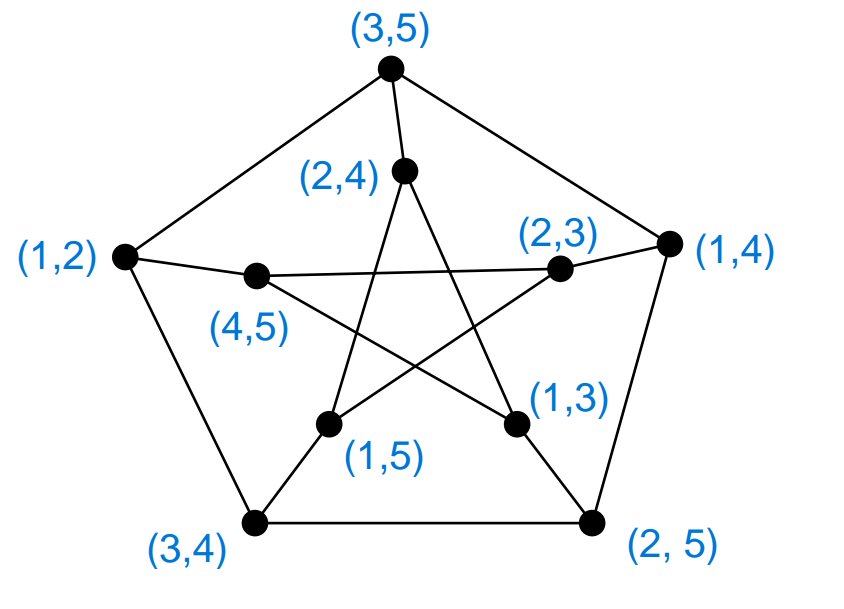
\includegraphics[width=7cm]{img/hw1/iso3}
                        \end{center}
            \end{enumerate}
      \item[3] \begin{enumerate}
                  \item The smallest one I could easily find has $|V|=6$:
                        \begin{center}
                              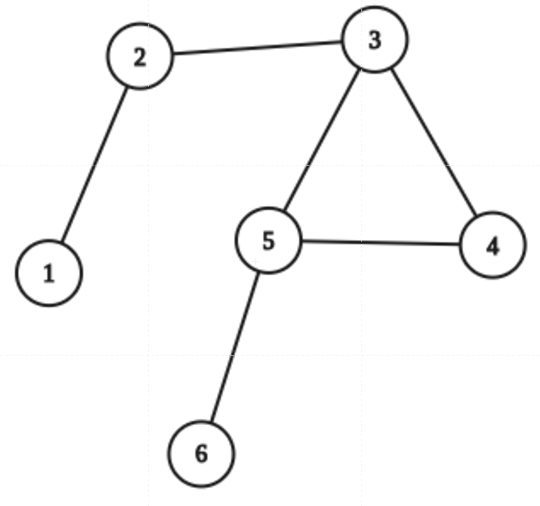
\includegraphics[width=5cm]{img/hw1/asymmetric}
                        \end{center}
                  \item I looked up all the graph isomorphisms with at most $5$ nodes
                        and found non-trivial automorphisms for all of them.
            \end{enumerate}
\end{enumerate}

\section{Chapter 4.2}

\begin{enumerate}
      \item[1] If $G$ is disconnected, then it has at least two connected components and
            we can split it into two nonempty sets of vertices with no edge between the two.
            Call the two sets $V_1$ and $V_2$.
            Notice that
            \[\forall v_1 \in V_1, v_2 \in V_2\ (v_1, v_2) \notin E \therefore (v_1, v_2) \in \binom{V}{2} \setminus E\]
            Now we WTS that for any pair of nodes there exists a path between them.
            There's a couple cases to consider if we wanna go from some node $s$ to some node $t$:
            \begin{itemize}
                  \item $s, t \in V_1$: we can go from $s$ to $x$ to $t$, where $x$ is any node in $V_2$.
                  \item $s, t \in V_2$: similarly, we can go from $s$ to $x$ to $t$, only this time $x$ is any node in $V_1$.
                  \item If $s \in V_1$ and $t \in V_2$: by our observation they are directly connected by an edge.
            \end{itemize}
            As we can see, we can find a path between any two nodes, making the complement of $G$ connected. $\square$

      \item[5] Besides a triangle, all cycles of length greater than $3$ are banned.
            This means our graph should either be a triangle with no other edges or a tree.
            We can't attach any edges to a triangle because then that would create a path of length $3$.

            The tree can have a maximum diameter of $2$,
            which restricts it to being a spider-like graph
            with a node in the center and nodes directly connected to it via edges.

            Any graph with max path length $3$ will only have either trees of the
            type just describes or triangles as connected components.
\end{enumerate}

\pagebreak

\section{Chapter 4.3}

\begin{enumerate}
      \item[1] The second and third graphs aren't isomorphic to the first one
            because they have a Hamiltonian \textit{cycle} while the first one doesn't.

            The second and third graphs themselves are also not isomorphic to each other,
            as the node distances are different.
            Notice that in the third, each node is $1$ edge away from exactly $3$ other nodes,
            $2$ edges away from $4$ other nodes, and $3$ edges away from $2$ other nodes.
            However, in the second graph there exists a node that doesn't follow
            these distances:
            \begin{figure}[h]
                  \centering
                  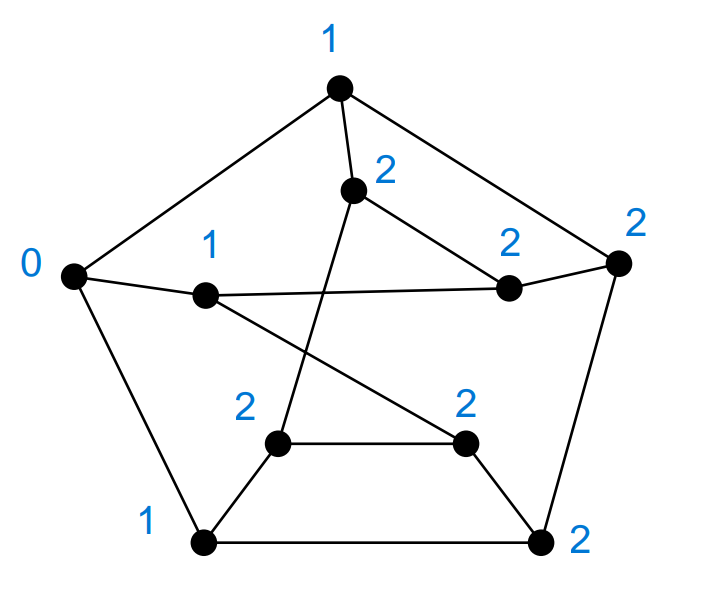
\includegraphics[width=6cm]{img/hw1/distance}
                  \caption{The node labelled $0$ is the one I'm taking distances from.}
                  \label{fig:distance}
            \end{figure}
            Thus, all three graphs are pairwise non-isomorphic. $\square$

      \item[9] Let us show that if I have a path of length $k < d$, I can extend it to form a path of length $k+1$.

            Say our path goes $n_0, n_1, \cdots, n_k$.
            $n_k$ has degree at least $d$, and $k<d$, so  by the pigeonhole
            principle we can always find an edge from $n_k$ to an $n_{k+1} \in V$
            that isn't already in the path.
            Adding $n_{k+1}$ onto our path gives us a new path of length $k+1$.

            Combined with the trivial base case of a path of length $1$,
            we can use this to iteratively construct a path of length $d$. $\square$
\end{enumerate}

\end{document}
